\documentclass[11pt,a4paper]{article}
\usepackage[utf8]{inputenc}
\usepackage[T1]{fontenc}
\usepackage{lmodern}
\usepackage[margin=24mm]{geometry}
\usepackage{amsmath,amssymb,graphicx,booktabs,tabularx,float}
\usepackage[protrusion=true,expansion=true]{microtype}
\usepackage[hidelinks]{hyperref}
\graphicspath{{relatorio/figuras/}}
\renewcommand{\abstractname}{Resumo}
\renewcommand{\figurename}{Figura}
\renewcommand{\tablename}{Tabela}
\renewcommand{\refname}{Referências}
\setlength{\parskip}{0.3em}
\setlength{\parindent}{1.15em}
\setlength{\emergencystretch}{1.25em}
\hypersetup{pdftitle={Resolução tridiagonal de sistemas não lineares de Broyden},pdfsubject={CI1164 - Método de Newton e análise de desempenho}}
\newcommand{\Autores}{} % Insira o nome dos integrantes e os logins do DInf.
% Gerado por benchmark/analise.py a partir das amostras registradas.
\newcommand{\ConstanteUltima}{1}
\newcommand{\Repeticoes}{10}
\newcommand{\EstadoRelatorio}{Ensaio preliminar}
\newcommand{\ResumoMedido}{Para $N=20000$, o tempo médio total passou de 6,249 para 2,761 ms no ensaio preliminar, com razão de 2,26 entre os tempos. A caracterização por contadores LIKWID está pendente.}
\newcommand{\AmbienteMedido}{As execuções foram fixadas na CPU lógica 2. O sistema identificou o processador AMD EPYC 9V45 96-Core Processor. O compilador foi \emph{gcc (Debian 14.2.0-19) 14.2.0}. A detecção de arquitetura do GCC selecionou \texttt{znver5}. Os recursos SIMD expostos incluem AVX, AVX2, AVX-512, FMA. O ambiente expõe 9 CPUs lógicas e a indicação de hipervisor. A hierarquia física de cache, a frequência efetiva e as condições de isolamento ficam indeterminadas para esta coleta. }
\newcommand{\ResultadosMedidos}{%
\begin{figure}[H]
\centering
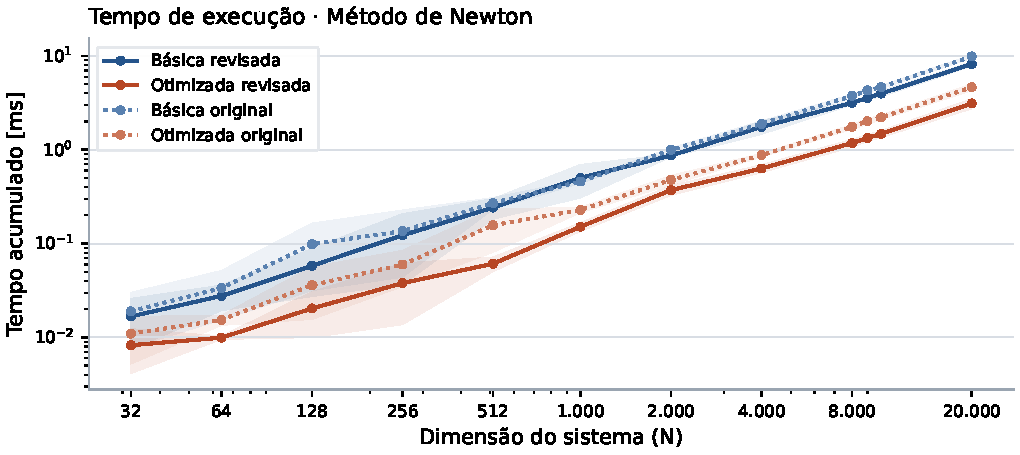
\includegraphics[width=0.88\linewidth]{tempo-newton_total.pdf}
\caption{Tempo de execução para o método de Newton. A faixa sombreada indica um desvio-padrão em torno da média.}
\end{figure}
Para $N=20000$, a baseline mediu 6,249 e a otimizada, 2,761. Os valores estão em ms para 25 passos. Em $N=32$, as médias foram 0,0143 e 0,0071 ms, respectivamente. O quociente de tempos baseline/otimizada em $N=20000$ foi 2,26. Na otimizada, dobrar $N$ de 10000 para 20000 multiplicou o tempo por 2,02. A curva agrega resíduo, Jacobiana, resolução linear e atualização. Em $N=32$, a baseline teve média de 0,0143 ms e mediana de 0,0117 ms. O desvio-padrão equivaleu a 57\% da média.

\begin{figure}[H]
\centering
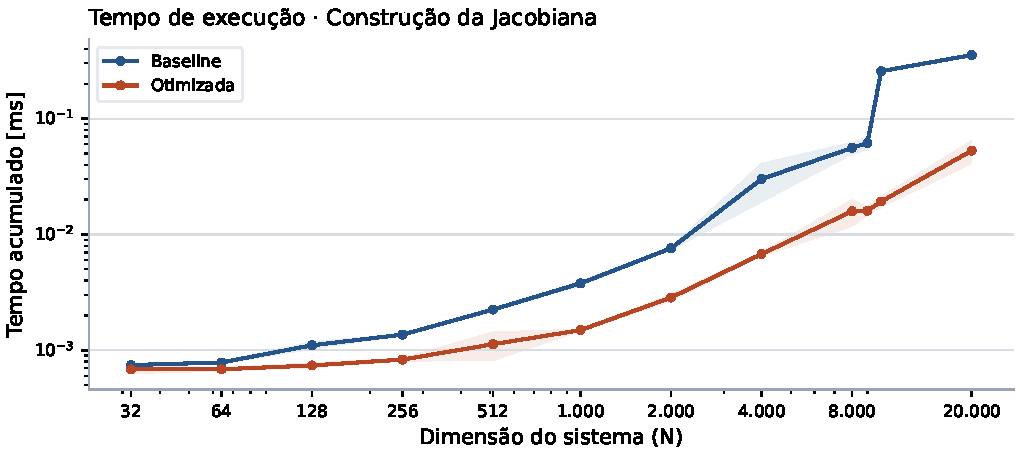
\includegraphics[width=0.88\linewidth]{tempo-jacobiana.pdf}
\caption{Tempo de execução para a construção da Jacobiana. A faixa sombreada indica um desvio-padrão em torno da média.}
\end{figure}
Para $N=20000$, a baseline mediu 0,354 e a otimizada, 0,053. Os valores estão em ms para 25 passos. Em $N=32$, as médias foram 0,0007 e 0,0007 ms, respectivamente. O quociente de tempos baseline/otimizada em $N=20000$ foi 6,69. Na otimizada, dobrar $N$ de 10000 para 20000 multiplicou o tempo por 2,75. A menor região é sensível à resolução do relógio e ao custo de chamada. Em $N=10000$, a baseline teve média de 0,2568 ms e mediana de 0,0727 ms. O desvio-padrão equivaleu a 225\% da média.

\begin{figure}[H]
\centering
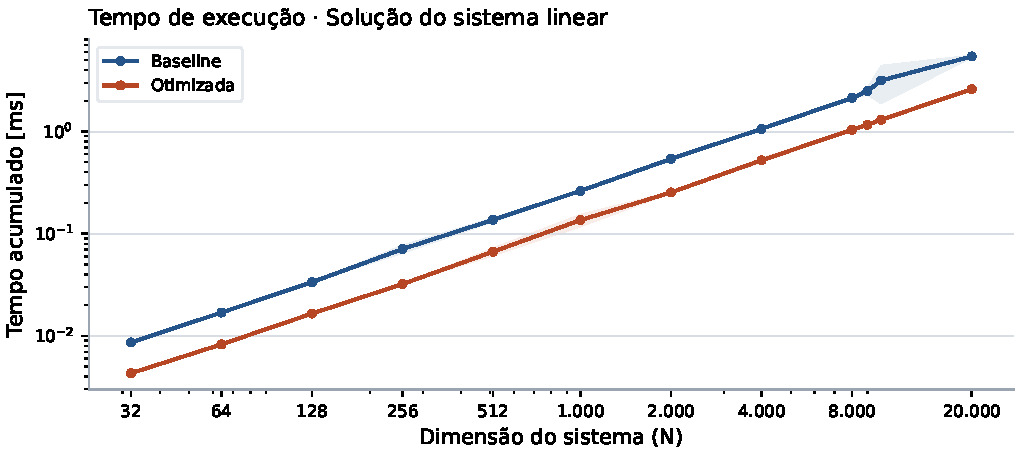
\includegraphics[width=0.88\linewidth]{tempo-sistema_linear.pdf}
\caption{Tempo de execução para a solução do sistema linear. A faixa sombreada indica um desvio-padrão em torno da média.}
\end{figure}
Para $N=20000$, a baseline mediu 5,448 e a otimizada, 2,606. Os valores estão em ms para 25 passos. Em $N=32$, as médias foram 0,0086 e 0,0043 ms, respectivamente. O quociente de tempos baseline/otimizada em $N=20000$ foi 2,09. Na otimizada, dobrar $N$ de 10000 para 20000 multiplicou o tempo por 1,99. A eliminação e a retrocessão mantêm dependências entre linhas vizinhas. Em $N=10000$, a baseline teve média de 3,1685 ms e mediana de 2,7372 ms. O desvio-padrão equivaleu a 41\% da média.

\subsection{Contadores pendentes}
A campanha ainda precisa de séries completas para \texttt{MEM}, \texttt{L2CACHE}, \texttt{FLOPS\_DP}, \texttt{FLOPS\_AVX}. 
As curvas correspondentes requerem a coleta dos contadores em um equipamento compatível.
}


\title{\textbf{Resolução tridiagonal de sistemas\\não lineares de Broyden}}
\author{\Autores\ifx\Autores\empty\else\\[3pt]\fi
  \small CI1164 -- Introdução à Computação Científica\\
  \small Departamento de Informática, Universidade Federal do Paraná}
\date{\small\EstadoRelatorio}

\begin{document}
\maketitle

\begin{abstract}
Estudamos a resolução do sistema tridiagonal de Broyden com o método de Newton. Comparamos as versões básica e otimizada do programa antes e depois de uma revisão. Todas calculam a Jacobiana analiticamente e usam tempo e memória lineares na dimensão do sistema por iteração. A revisão forma o lado direito em uma passagem e intercala duas recorrências de eliminação a partir das extremidades do sistema quando os pivôs têm uma garantia de magnitude. \ResumoMedido
\end{abstract}

\noindent\textbf{Palavras-chave}\quad Método de Newton, Jacobiana tridiagonal, pivotamento parcial, LIKWID.

\section{Introdução}

O método de Newton para sistemas não lineares resolve um sistema linear a cada passo. O custo de uma implementação depende da forma de representar a Jacobiana e do algoritmo adotado para resolver esses sistemas. O problema de Broyden oferece uma estrutura conhecida que permite comparar duas implementações seriais com a mesma ordem de complexidade. Avaliamos a contribuição da construção da Jacobiana e do solucionador linear no tempo das 25 atualizações.

\section{Formulação}

Seja $X=(x_1,\ldots,x_N)^T$. A função usada é
\begin{equation}
F_i(X)=(3-2x_i)x_i-x_{i-1}-2x_{i+1}+c_i,\qquad 1\le i\le N,
\label{eq:broyden}
\end{equation}
com vizinhos de contorno $x_0=x_{N+1}=0$, $c_i=1$ para $i<N$ e $c_N=\ConstanteUltima$. O símbolo $x_0$ usado no enunciado para a entrada designa o valor inicial comum de $x_1,\ldots,x_N$. Os vizinhos de contorno da equação~\eqref{eq:broyden} são constantes distintas do valor inicial.

A função clássica de Moré, Garbow e Hillstrom~\cite{more} usa $c_N=1$. O gerador preservado no primeiro commit omite o termo constante na última linha. A cópia local do gerador inclui o termo. A figura oficial ainda é necessária para confirmar a equação adotada na correção. A opção \texttt{LAST\_CONSTANT} do Makefile permite reproduzir ambas as variantes. A campanha usa a mesma variante em todos os binários.

Em cada passo $k$,
\begin{equation}
J(X^{(k)})\,\Delta X^{(k)}=-F(X^{(k)}),\qquad
X^{(k+1)}=X^{(k)}+\Delta X^{(k)}.
\end{equation}
A Jacobiana tem diagonal $d_i=3-4x_i$, subdiagonal $-1$, superdiagonal $-2$ e zeros fora da banda. Com tolerância positiva, o programa testa $\|F(X^{(k)})\|_\infty\le\epsilon$ antes de montar a Jacobiana. A norma do resíduo usa máximo dos módulos. Uma correção pequena pode indicar estagnação e, sozinha, é insuficiente para aceitar o vetor. Com $\epsilon=0$, o laço executa até \texttt{MAX}, sujeito a uma falha numérica diagnosticada. A execução com \texttt{MAX=0} imprime o vetor inicial e tempos zerados.

\section{Implementação e otimizações}

\subsection{Eliminação em banda}

A versão básica usa pivoteamento parcial adjacente. Em cada coluna, a eliminação compara o pivô corrente com o elemento imediatamente abaixo dele, cujo valor é $-1$. A revisão dispensa a inicialização e a leitura da subdiagonal. Uma troca pode criar uma segunda superdiagonal, que ocupa o vetor reservado anteriormente para a subdiagonal. Uma vez processada cada coluna, o pivô tem módulo maior ou igual a 1. Na retrocessão, apenas o último pivô precisa de uma checagem adicional. O esquema de trocas partilha a estrutura matemática da rotina DGTSV~\cite{lapack}.

A otimizada examina a condição suficiente $|d_i|\ge 3$ com valores finitos. Escrevendo $b=-F(X)$, a versão original eliminava da primeira até a última linha. A versão revisada aplica a recorrência de Thomas de cada extremidade em direção a uma equação central. À esquerda, o pivô e o termo independente normalizado são
\begin{align*}
p_1 &= d_1, & w_1 &= b_1/p_1,\\
p_i &= d_i-2/p_{i-1}, & w_i &= (b_i+w_{i-1})/p_i, \qquad i\ge2.
\end{align*}
À direita, a correção do pivô continua sendo $2/p_{i+1}$, enquanto o termo normalizado é $(b_i+2w_{i+1})/p_i$. Como $|d_i|-2/|p_{i\pm1}|\ge2$ quando $|p_{i\pm1}|\ge2$, os pivôs laterais têm módulo pelo menos 2. Na linha central, as duas correções juntas têm módulo de no máximo 2. Seu pivô tem módulo de pelo menos 1. A retrocessão parte da solução central. Cada linha à esquerda usa o coeficiente $2/p_i$ e cada linha à direita, $1/p_i$, já armazenados nos vetores do sistema. A rotina usa uma divisão por linha. As duas cadeias independentes permitem intercalar instruções escalares. Se a verificação inicial falhar, a otimizada usa o mesmo pivoteamento da básica.

\subsection{Acesso à memória e vetorização}

O material de otimização disponível da disciplina inclui um exemplo de produto de matrizes e scripts de coleta. As técnicas aqui avaliadas incluem acesso sequencial, redução de passagens por vetores, independência entre operações e vetorização pelo compilador. O PDF dos slides e a figura do enunciado seguem pendentes.

\begin{table}[H]
\centering
\small
\begin{tabularx}{\linewidth}{@{}p{0.30\linewidth}X@{}}
\toprule
Trecho & Técnica e efeito esperado \\
\midrule
\texttt{calcMenosF} & Forma o lado direito diretamente. Na otimizada, as fronteiras ficam fora do laço interno e os vizinhos são acessados em posições consecutivas. \\
\texttt{calcJ} & Vetores contíguos e diagonal analítica. A região da Jacobiana escreve $N$ coeficientes em ambas as versões. \\
\texttt{eliminacaoGauss} & A subdiagonal é implícita. O caminho de Thomas intercala duas cadeias de divisões e guarda os coeficientes da retrocessão. \\
\texttt{atualizaX} & Atualização e checagem de finitude em uma passagem. A troca de ponteiros reutiliza o vetor anterior como área de trabalho. \\
\texttt{alocaVetores} & Uma alocação antes do laço com fatias alinhadas a 64 bytes na versão otimizada. O uso de \texttt{restrict} expressa que as fatias lidas e escritas são disjuntas. \\
\bottomrule
\end{tabularx}
\caption{Otimizações aplicadas aos trechos computacionais.}
\end{table}

As duas versões reservam cinco vetores de \texttt{double} em uma área contígua, com arredondamento dos comprimentos na otimizada para alinhar o início de cada vetor. Com $N=20000$, a reserva soma 800\,000 bytes por versão. O caminho de Thomas acessa três vetores, totalizando 480\,000 bytes de dados distintos no passo de Newton. As duas fatias restantes estão disponíveis para o caminho com pivotamento. Uma Jacobiana densa conteria $N^2$ elementos e reservaria 3,2 GB nesse tamanho. Materializá-la exigiria $\Theta(N^2)$ escritas e usar eliminação densa exigiria $\Theta(N^3)$ operações. Calcular diferenças finitas coluna a coluna com uma avaliação de $F$ para cada perturbação também custaria $\Theta(N^2)$ operações. Na implementação escolhida, resíduo, Jacobiana, solução linear e atualização custam $\Theta(N)$ por passo e o armazenamento de trabalho é $\Theta(N)$.

O GCC informou vetorização com vetores de até 32 bytes para os laços do resíduo otimizado, da diagonal, da checagem para Thomas e da atualização. O solucionador usa divisões escalares. Dentro de cada metade, o pivô e o lado direito reduzido dependem da linha anterior. O trabalho na outra metade pode ser intercalado no mesmo núcleo. As verificações de finitude continuam ativas.

\subsection{Ensaios isolados de otimização}

Em uma rodada intercalada com dez repetições, $N=20000$ e todos os estágios compilados com as mesmas opções, o tempo médio da região linear passou de 3,538 para 1,986 ms com a eliminação pelas duas pontas. Na básica, a simplificação do pivoteamento reduziu a região linear de 8,231 para 6,823 ms. A formação direta de $-F(X)$ eliminou uma passagem, com diferença de tempo total pequena nesta amostra. A remoção do alinhamento elevou a média da Jacobiana de 0,304 para 0,406 ms. Mantivemos o alinhamento e usamos \texttt{-ffp-contract=fast} em todos os estágios.

\section{Validação numérica}

Um teste de kernels comparou a Jacobiana com diferenças centrais para cada entrada de uma matriz de dimensão cinco. Três sistemas com solução construída exercitaram dominância e trocas de linha, incluindo candidatos a pivô de magnitude $10^{-16}$. Um segundo conjunto comparou cada passo de Newton em dimensão até dez com eliminação densa independente, aferiu $J\Delta X+F(X)$ e confirmou os vetores finais das duas versões em 22 casos válidos. O conjunto também cobriu dimensões de 1 a 20000, entradas inválidas, falhas de alocação induzidas com limite de memória, casos singulares e resultados não finitos.

Com $x_i^{(0)}=-1$, $\epsilon=0$ e \texttt{MAX=25}, ambas as versões completaram 25 atualizações em todos os tamanhos. O maior resíduo final verificado para a formulação clássica ficou abaixo de $1{,}4\times 10^{-15}$ nas duas versões. Os testes com AddressSanitizer e UndefinedBehaviorSanitizer passaram. A verificação de vazamentos do LeakSanitizer exigia recursos ausentes no ambiente virtual e foi desabilitada nessa execução.

\section{Metodologia experimental}

\AmbienteMedido

As duas versões foram compiladas com GCC na máquina de medição. A baseline e a otimizada receberam as opções \texttt{-O3 -march=native -mavx -fopt-info-vec}. Os sistemas das duas versões usam os mesmos valores de entrada, $x_i^{(0)}=-1$, $\epsilon=0$, \texttt{MAX=25} e
\begin{equation*}
 N\in\{32,64,128,256,512,1000,2000,4000,8000,9000,10000,20000\}.
\end{equation*}
Foi executado um aquecimento por ponto e por versão, seguido de \Repeticoes{} repetições em processos independentes. Os tamanhos foram embaralhados com semente fixa e a versão executada primeiro alternou entre os pares. Os resultados são a média das amostras de cada configuração. A dispersão, a mediana e os extremos também são preservados no CSV.

Os tempos vêm de \texttt{timestamp()}, em milissegundos, sem ativação do LIKWID nesta família de medições. O programa acumula separadamente o intervalo computacional de cada passo e os intervalos para montar $J$ e resolver o sistema linear. Inicialização, formatação e escrita de vetores ocorrem fora desses intervalos. O descarte para \texttt{/dev/null} evita armazenamento da saída e mantém a formatação real entre passos, com possível efeito sobre o estado do cache.

Nos binários instrumentados, a região \texttt{Newton\_Total} contém os marcadores \texttt{Jacobiana} e \texttt{Sistema\_Linear}. Registramos os nomes uma vez e os marcadores são acionados por passo. O LIKWID acumula leituras sobre chamadas sucessivas~\cite{likwid}. O coletor valida 25 chamadas de cada região na CPU selecionada e salva a saída nativa antes de extrair as métricas. O custo da instrumentação das regiões internas integra a medição do marcador externo. Em regiões curtas, chamadas do relógio, dos marcadores e variação da frequência podem ter peso relevante~\cite{pitfalls}.

O fabricante identifica esse modelo como Kaby Lake~\cite{intel}. O LIKWID 5.4.1 leu a topologia, mas o acesso a contadores falhou com \texttt{perf\_event\_paranoid=3}. A campanha tentou banda de memória de \texttt{MEM} em MB/s, razão de faltas de \texttt{L2CACHE} e taxas em MFLOP/s de \texttt{FLOPS\_DP} e \texttt{FLOPS\_AVX}. Também sondou \texttt{L3}, \texttt{L1CACHE} e \texttt{CACHE}. Nenhuma tentativa retornou amostras de hardware.

\section{Resultados}

\ResultadosMedidos

\section{Discussão}

Definimos a aceleração como a razão entre as médias de tempo da baseline e da otimizada. Como as duas versões têm complexidade linear, a comparação avalia diferenças na quantidade de operações, no tráfego de dados e no código produzido pelo compilador. A região do sistema linear executa um laço de eliminação com uma dependência de divisão e outro de retrocessão com dependência de leitura da correção vizinha. A construção da Jacobiana consiste em poucos cálculos e uma passagem por um vetor, o que torna a medição em dimensões pequenas sensível a custos fixos. O desvio-padrão mostrado nos gráficos ajuda a avaliar essas duas situações.

Para $N=20000$, a revisão melhorou o tempo de Newton da básica em $1{,}21\times$ e o da otimizada em $1{,}49\times$. O sistema linear representou 75\% do tempo computacional da otimizada original e 64\% na revisada. O tempo médio da Jacobiana otimizada subiu de 0,312 para 0,360 ms, com desvios-padrão de 0,085 e 0,111 ms. A implementação de \texttt{calcJ} foi preservada. A comparação de tempos de parede da otimizada apresentou medianas de 131,21 e 131,51 ms. O custo de formatar 520 mil linhas de variáveis ajuda a explicar por que o ganho computacional pouco aparece no tempo de parede.

O efeito de cache depende dos tamanhos e associatividade disponíveis na CPU de teste, do reuso entre regiões e dos acessos do processo que escreve os vetores. Banda de memória é uma taxa de transferência. Para investigar se uma banda maior veio de mais tráfego, também é necessário examinar o volume e a duração da região. A interpretação de MFLOP/s depende dos eventos que contam operações escalares, vetoriais e instruções fundidas. Uma aceleração pode vir da eliminação de operações e corresponder a uma taxa aritmética menor. Um estudo Roofline requer banda e trabalho de ponto flutuante medidos no ambiente da campanha.

\section{Conclusão}

A construção analítica e a exploração da banda permitem resolver cada passo em tempo e memória $\Theta(N)$. O pivotamento adjacente cobre entradas fora da condição suficiente de Thomas e os testes com casos construídos confirmaram a operação da retrocessão após as trocas. As séries de tempo permitem comparar as duas implementações por região. A validação da última equação contra a figura do enunciado e a cobertura dos contadores estão documentadas junto à formulação e aos resultados.

\begin{thebibliography}{9}
\raggedright
\bibitem{more} MORÉ, J. J., GARBOW, B. S. e HILLSTROM, K. E. \emph{Testing Unconstrained Optimization Software}. ACM Transactions on Mathematical Software, v. 7, n. 1, p. 17--41, 1981. \url{https://doi.org/10.1145/355934.355936}.
\bibitem{intel} INTEL. \emph{Core i5-7500 Processor Specifications}. \url{https://www.intel.com/content/www/us/en/products/sku/97123/intel-core-i57500-processor-6m-cache-up-to-3-80-ghz/specifications.html}.
\bibitem{lapack} LAPACK. \emph{DGTSV, solução de sistemas tridiagonais com pivotamento parcial}. Netlib. \url{https://www.netlib.org/lapack/explore-html/d6/ddb/group__gtsv_ga6b06a11b8e2dced10bc9cd3c20a09484.html}.
\bibitem{likwid} RRZE-HPC. \emph{likwid-perfctr e Marker API}. \url{https://github.com/RRZE-HPC/likwid/wiki/likwid-perfctr}.
\bibitem{pitfalls} RRZE-HPC. \emph{LikwidMarkerAPIPitfalls}. \url{https://github.com/RRZE-HPC/likwid/wiki/LikwidMarkerAPIPitfalls}.
\end{thebibliography}
\end{document}
